\chapter{Introdução}\label{cap:cap1}

\begin{flushright}
  \textit{
    Persistência é a irmã gêmea da excelência. \\
    Uma é a mãe da qualidade, a outra é a mãe do tempo.
  } \\
  
  \textbf{Marabel Morgan}
\end{flushright}


Antes de prosseguir com a disciplina, é importante que tenhamos uma compreensão clara e detalhada dos conceitos relacionados à \textbf{Orientação a Objetos (POO)}. Esses conceitos incluem \textbf{Classes, Métodos, Herança, Objetos} e outros conceitos interligados. A compreensão desses conceitos é fundamental para podermos aproveitar ao máximo as vantagens do paradigma da Orientação a Objetos e utilizá-lo de maneira efetiva na solução de problemas complexos. É através da compreensão desses conceitos que poderemos desenvolver soluções mais organizadas, claras e eficientes. Por isso, este capítulo introdutório visa apresentar esses conceitos de concisamente, proporcionando uma base sólida para o desenvolvimento de habilidades e conhecimentos mais avançados no decorrer da disciplina. Então, estejam atentos e preparem-se para mergulhar no mundo da Orientação a Objetos.

\section{Orientação a objeto}

O Paradigma da Orientada a Objetos (também conhecida pela sua sigla POO) pretende representar o mais fielmente possível as situações reais nos sistemas computacionais. Nós entendemos o mundo todo composto por vários objetos que interagem uns com os outros. Da mesma maneira, a Orientação a Objetos consiste em considerar os sistemas computacionais não como uma coleção estruturada de processos, mas sim como uma coleção de objetos que interagem entre si \cite{farinelli2007conceitos}.

\begin{figure}[H]
	\centering
	\caption{Um sistema constituído de objetos que interagem entre si.}
	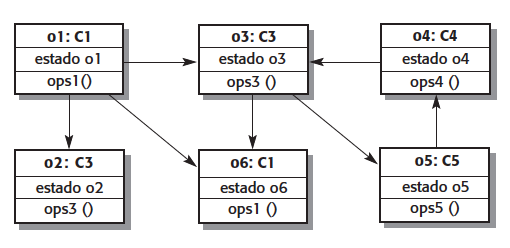
\includegraphics[scale=0.6]{imagens/figura-01.png}
	\legend{Fonte: \cite{sommerville2003engenharia}}
	\label{fig:figura-01}
\end{figure}

Segundo Peter Van Roy, um paradigma de programação define como a programação é realizada. Cada paradigma possui seu próprio conjunto de técnicas e formas de estruturar o pensamento na composição de software \cite{vanroy2012}. Cada paradigma tem suas próprias vantagens e desvantagens e o desenvolvedor deve escolher o mais adequado para cada projeto e problema a ser resolvido.

\begin{figure}[H]
	\centering
	\caption{Paradigmas de Programação.}
	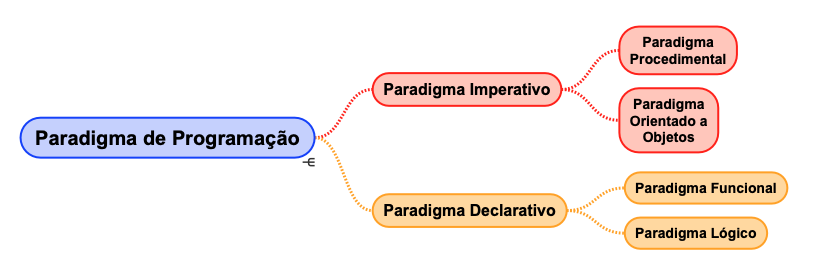
\includegraphics[scale=0.5]{imagens/paradigmas.png}
	\legend{Fonte: O Autor }
	\label{fig:paradigmas}
\end{figure}

A programação orientada a objetos (POO) é um dos quatro principais paradigmas de programação, com o procedimental, funcional e lógico. A POO é uma abordagem para projetar e desenvolver software que se concentra na representação de entidades reais como objetos, com atributos e comportamentos. A programação orientada a objetos é realizada utilizando uma linguagem de programação orientada a objetos, como Java, que permite a implementação direta de objetos e fornece recursos para definir classes de objetos, como seus atributos e métodos. Esta abordagem permite a criação de programas de software mais organizados, reutilizáveis e fáceis de manter. A POO é amplamente utilizado em aplicações comerciais, games, sistemas web e muitos outros categorias de software, devido à sua capacidade de representar conceitos complexos de uma forma simples e fácil de entender. Além disso, a POO permite a reutilização de código, tornando o desenvolvimento de software mais rápido e eficiente \cite{sommerville2003engenharia}.

\section{Principais conceitos de POO}

A Programação Orientada a Objetos (POO), como já visto, é um paradigma de programação que se concentra em modelar conceitos reais como objetos computacionais, dotados de características e comportamentos. Esta abordagem permite a representação de dados e ações de forma mais intuitiva e natural, proporcionando uma melhor organização e reutilização de código em projetos de software. Abaixo será apresentado alguns dos principais conceitos envolvidos no paradigma.

\subsection{Classes e objeto}

Para \cite{sommerville2003engenharia} ``objeto'' e ``orientado a objetos'' são
amplamente utilizados e aplicados a diferentes categorias de entidades, métodos de
projeto, sistemas e linguagens de programação. Contudo, existe uma aceitação
geral de que um objeto é um encapsulamento de informações, e isso se reflete na
definição de um objeto e de uma classe de objeto a seguir:

\begin{itemize}
  \item Um objeto é uma entidade que possui um estado e um conjunto definido de
  operações que operam nesse estado. O estado é representado por um conjunto de
  atributos de objeto. As operações associadas com o objeto fornecem serviços para outros objetos (clientes), que requisitam esses serviços quando alguma computação é necessária.

  \item Os objetos são criados de acordo com uma definição de classe de objetos 
  que serve como um template para criar objetos. Essa classe apresenta 
  declarações de todos os atributos e operações que devem ser associados a um 
  objeto dessa classe.
\end{itemize}

Em outras palavras, pode-se dizer que classe é uma descrição generalizada que
descreve uma coleção de objetos similares, o qual, segundo 
\citeonline{pressman2016engenharia}, é um conceito orientado a objeto que 
encapsula dados e abstrações procedurais necessárias para descrever o conteúdo 
e comportamento de alguma entidade real.

Exemplos de objetos são: os \textbf{objetos físicos} (um livro, uma caneta), \textbf{funções de pessoas} para os sistemas (funcionário, cliente), \textbf{eventos} (uma compra, um  telefonema), \textbf{interações} entre outros objetos (um item de uma nota fiscal é uma interação entre uma compra e um produto do estoque) e \textbf{lugares} (loja matriz, revenda nordeste).

Para fins de estudo, e com objetivo mais didático, usaremos um cachorro como 
nosso ``objeto'':

\begin{figure}[H]
  \centering
  \caption{Representação de um objeto}
  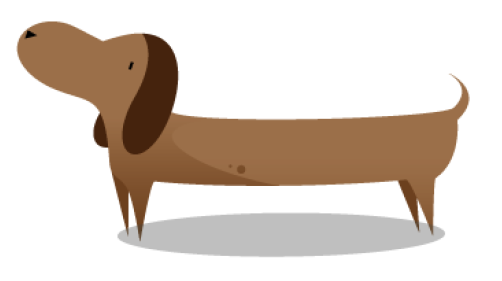
\includegraphics[scale=0.4]{imagens/cachorro-objeto.png}
  \caption{\textbf{Fonte:} O autor}
  \label{fig:cachorro-objeto}
\end{figure}

Ao analisar o objeto, deduz-se que há características pertencentes somente a 
ele. Tais como:

\begin{itemize}
  \item Nome;
  \item Idade;
  \item Comprimento de pelos;
  \item Cor dos pelos;
  \item Cor dos olhos;
  \item Peso, entre outros;
\end{itemize}

Tais características que descrevem um objeto são chamadas na orientação a  objeto de atributos.

\subsection{Atributos}

Os objetos reais têm propriedades que, no que lhe concerne, possuem valores. 
Estes valores determinam o \textbf{estado do objet}o. Assim, na orientação a objeto, 
essas propriedades são chamadas atributos. Logo, podemos dizer que esses atributos são como variáveis ou campos que guardam os variados valores que os objetos podem receber como características.

\textbf{O estado de um objeto é um grupo de valores que estão em seus atributos em um certo momento}. \\

\begin{minipage}{\textwidth}
  \begin{minipage}[b]{0.49\textwidth}
    \centering
    \captionof{figure}{Representação de um objeto}    
    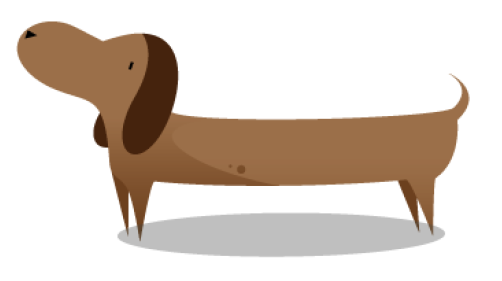
\includegraphics[scale=0.4]{imagens/cachorro-objeto.png}
    \caption*{\textbf{Fonte:} O autor}    
    \label{fig:cachorro-objeto-1}
  \end{minipage}
  \hfill
  \begin{minipage}[b]{0.52\textwidth}
    \centering
    \captionof{table}{Atributos e valores}
    \begin{tabular}{|l|l|}
      \hline
      \multicolumn{2}{|c|}{Cachorro}      \\ \hline
        Nome:                 & Hubert    \\ \hline
        Idade:                & 2 anos    \\ \hline
        Tipo Pelo:            & Curtos    \\ \hline
        Cor dos pelos:        & Marrom    \\ \hline
        Cor dos olhos:        & Castanhos \\ \hline
        Peso                  & 5kg       \\ \hline
      \end{tabular}
      \caption*{\textbf{Fonte:} O autor}  
    \end{minipage}
  \end{minipage} \\

  Outro objeto cachorro teria valores diferentes para estes mesmos atributos, como exemplo disto temos:

  \begin{minipage}{\textwidth}
    \begin{minipage}[b]{0.49\textwidth}
      \centering
      \captionof{figure}{Representação de um objeto}
      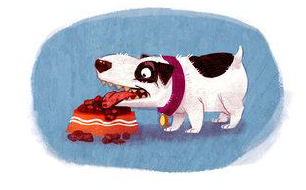
\includegraphics[scale=0.6]{imagens/cachorro-objeto-2.png}
      \caption*{\textbf{Fonte:} O autor}
      \label{fig:cachorro-objeto-2}
    \end{minipage}
    \hfill
    \begin{minipage}[b]{0.49\textwidth}
      \centering
      \captionof{table}{Atributos e valores}
      \begin{tabular}{|l|l|}
        \hline
        \multicolumn{2}{|c|}{Cachorro}      \\ \hline
          Nome:                 & Floks     \\ \hline
          Idade:                & 4 anos    \\ \hline
          Tipo pelo:            & Curtos    \\ \hline
          Cor dos pelos:        & Branco    \\ \hline
          Cor dos olhos:        & Castanhos \\ \hline
          Peso                  & 5kg       \\ \hline
        \end{tabular}
        \caption*{\textbf{Fonte:} O autor}
      \end{minipage}
    \end{minipage} \\ 

Para que os atributos de um objeto mudem de valor isso deve ser feito  exclusivamente por estímulos externos ou internos. Assim, a única maneira  de alterar os atributos dos objetos é disparando eventos que geram a mudança desses estados no objeto.

\subsection{Métodos}

Os métodos são uma parte fundamental dos objetos em programação. Eles são procedimentos ou funções que executam ações específicas e permitem que o objeto se manifeste e interaja com outros objetos. Esses métodos são acionados por mensagens enviadas por outros objetos, que solicitam a realização de uma ação específica. Os métodos também são responsáveis por acessar e modificar os atributos do objeto.

Como exemplo, no estudo de um objeto "cachorro", podemos identificar uma série de métodos que ele possui, como latir, babar, comer e sentar. Esses métodos são o comportamento que o objeto cachorro pode exibir quando estimulado por outro objeto. Em resumo, os métodos são as ações que o objeto consegue realizar, e é através deles que ele se manifesta e interage no mundo virtual.

Já em sistemas computacionais, os métodos são funções ou procedimentos definidos em classes, ou objetos e executam tarefas específicas. Eles são utilizados para encapsular lógica de negócios, processamento de dados e outras operações que um objeto precisa realizar. Em resumo, eles são uma parte fundamental da programação orientada a objetos e são amplamente utilizados em sistemas computacionais para ajudar a organizar e modularizar o código, além de permitir a interação e reutilização de objetos.

\subsection{Herança}\label{subsection:heranca}

O conceito de herança é um dos conceitos fundamentais de POO. Herança, na prática, significa a possibilidade de construir objetos especializados que herdam as características de objetos mais generalistas, ou ainda, a herança uma maneira de reutilizar código a medida que podemos aproveitar os atributos e métodos de classes já existentes para gerar novas classes mais específicas que aproveitarão os recursos da classe hierarquicamente superior \cite{evandroeduardoseronruiz2008}.

O conceito de herança mimetiza as características hierárquicas de vários sistemas reais, como, por exemplo, os sistemas de classificação em biologia que, pode determinar como uma hierarquia o seguinte:

\begin{itemize}
    \item animais;
    \item vertebrados e invertebrados;
    \item mamíferos e aves;
    \item entre outras características mais específicas
\end{itemize}

\begin{figure}[H]
  \centering
  \caption{Diagrama representando a herança entre as classes}
  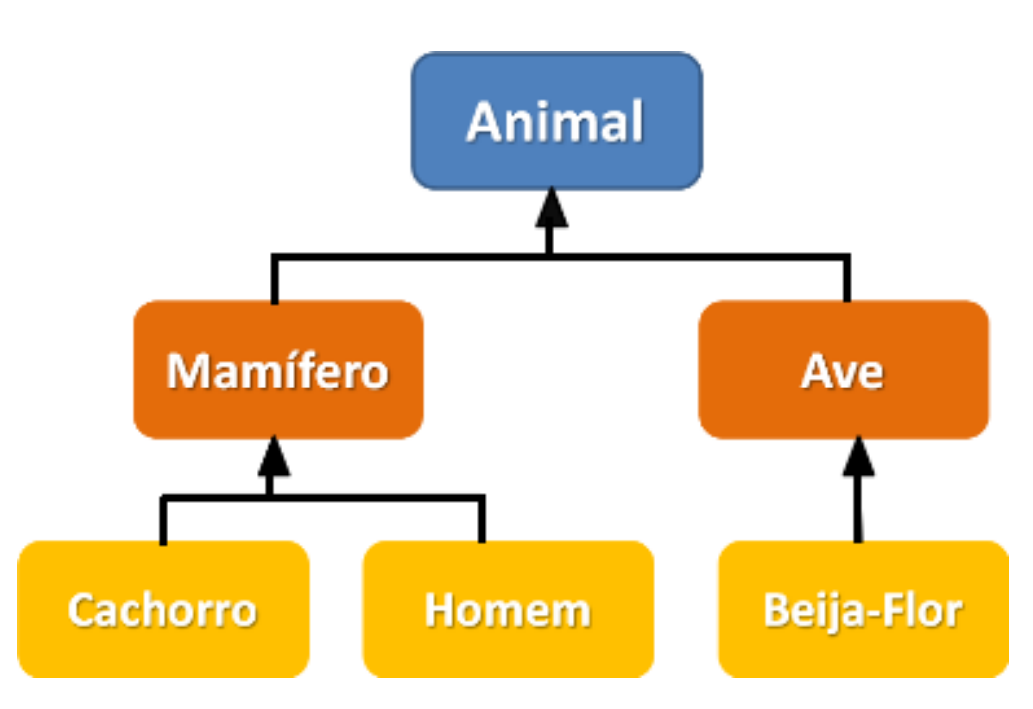
\includegraphics[scale=0.3]{imagens/heranca.png}
  \caption*{\textbf{Fonte:} ...}
  \label{fig:heranca}
\end{figure}

\section{Classes abstratas}

As classes abstratas são moldes para outras classes que herdam seus atributos e métodos. Elas não podem ser instanciadas diretamente, mas precisam ser estendidas por uma classe mais específica, a qual pode ser instanciada. Os métodos da classe abstrata precisam ser redefinidos nas classes filhas (subclasses), permitindo a personalização do comportamento do objeto. 

\begin{figure}[H]
	\centering
	\caption{Diagrama representando uma classe abstrata}
	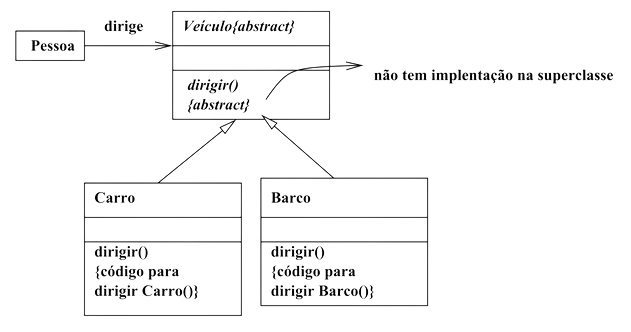
\includegraphics[scale=0.6]{imagens/classe-abstrata.png}
	\caption*{\textbf{Fonte}: \url{https://pt.slideshare.net/CristianoSilva11/class-abstrata-java}}
	\label{fig:abstrata}
\end{figure}

\subsection{Superclasses e subclasses}

Em POO todo objeto de uma classe construída pelo usuário da linguagem é também um objeto de outra classe. Por exemplo, na hierarquia de uma empresa, podemos dizer que pessoa é uma superclasse e que funcionário é uma subclasse de pessoa.

Outra nomenclatura utilizada para especificar superclasses ou subclasses é a Generalização, ou Especialização. No exemplo abaixo, pessoa é a generalização de empregado, e empregado é a especialização de pessoa conforme representado na Figura \ref{fig:sub-e-sup-classes}

Uma máxima que podemos guardar é: 

\begin{center}
\textbf{\textit{Uma subclasse guarda a relação é um com a superclasse.}}    
\end{center}

\begin{figure}[H]
  \centering
  \caption{Superclassses e Subclasses}
  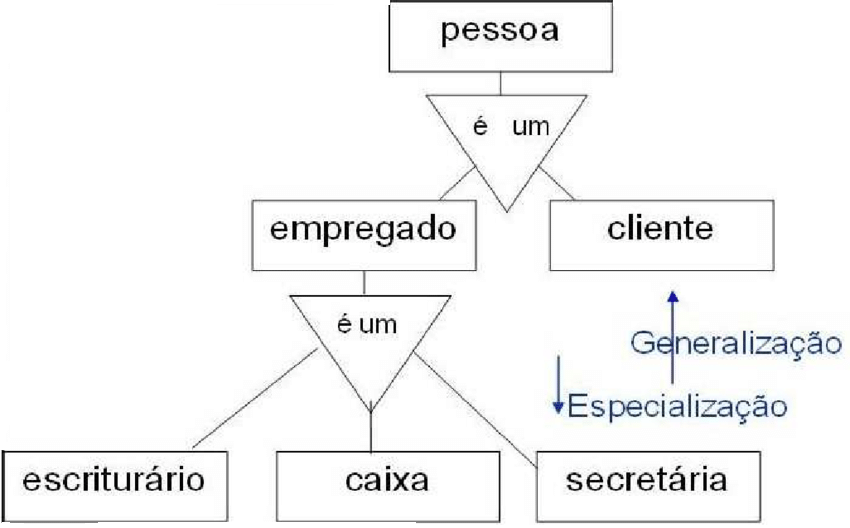
\includegraphics[scale=0.5]{imagens/sub-e-sup-classes.png}
  \legend{\textbf{Fonte}: \cite{articlelucas2009}}
  \label{fig:sub-e-sup-classes}
\end{figure}

\section*{Exercícios de fixação}\label{exer:001}

\begin{enumerate}
    \item Para satisfazer as necessidades de informatização de uma biblioteca universitária um sistema foi proposto para satisfazer algumas características:

\begin{itemize}
  \item Cadastro dos usuários da biblioteca com endereço completo. 
  Usuário são classificados em três grupos: professores, alunos e funcionário.  
  \item Cadastro das obras da biblioteca são classificados em: livros científicos, periódicos científicos, periódicos informativos, periódicos diversos, entretenimento, etc.
  \item Linguagem usada no exemplar da obra.
  \item Mídia que armazena o exemplar da obra.
  \item Autores da obra com o controle da nacionalidade dos mesmos.
  \item Editoras dos exemplares com ano de edição referente a cada exemplar.
\end{itemize}

Identifique os possíveis objetos com seus respectivos atributos e métodos.

\item \textbf{Desafio - Obrigatório:} Pesquise sobre os pontos negativos da orientação a objeto, principalmente sobre os conceitos que relacionam \textbf{Coesão} e \textbf{Acoplamento}.
\end{enumerate}

\section{Mensagem}

Mensagens são requisições enviadas de um objeto para outro, para que o objeto ``receptor'' forneça algum resultado desejado por meio da execução de uma operação. As trocas de mensagem funcionam como uma fábrica que
recebe uma ordem de produção (mensagem de solicitação), processa essa ordem (operações) utilizando matéria-prima (atributos) e gera um produto final (mensagem de resposta).

\begin{figure}[H]
  \centering
  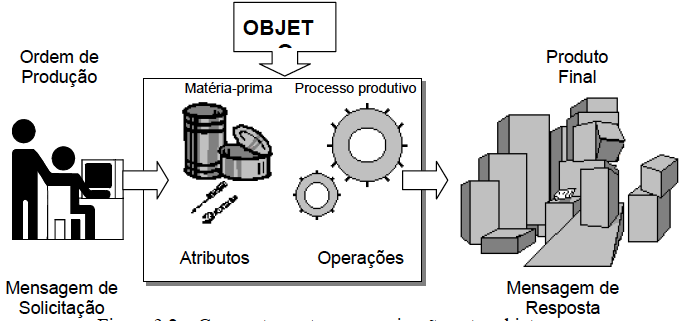
\includegraphics[scale=0.5]{imagens/analogia-mensagens.png}
  \caption{Comportamento e comunicação entre objetos}
  \label{}
\end{figure}

\section{Encapsulamento}

Cada objeto é visto como o encapsulamento do seu estado interno, suas mensagens e seus métodos. A estrutura do estado e dos pares "mensagem - método" são todas definidas através da classe à qual o objeto pertence.

\begin{itemize}
  \item A encapsulação de dados com o código que os manipula em classes é a principal vantagem da Orientação a Objeto
  \item No sentido de não quebrar a encapsulação, é muito importante que os membros de uma classe (atributos e métodos) sejam visíveis apenas onde estritamente necessário (A lei é: "Não posso quebrar o que não posso acessar").
\end{itemize}

\subsection{Especificadores de controle de acesso}

Com a ideia de encapsulamento nós também possuímos os especificadores de controle de acesso ou visibilidades. A visibilidade é a maneira com a qual o desenvolvedor proíbe ou permite acesso a determinados métodos, ou atributos de uma classe, como pode ser visto na Figura \ref{fig:encapsulamento}. Neste sentido, o objeto formado possuirá as mesmas definições declaradas pela classe.

\subsubsection{A visibilidade \textit{public}}
\begin{itemize}
  \item Quem tem acesso à classe tem acesso também a qualquer membro com visibilidade public;
  \item O alvo aqui é o programador cliente que usa suas classes;
  \item É raro ter atributos públicos, mas é comum ter métodos públicos.
\end{itemize}

\subsubsection{A visibilidade \textit{private}}
\begin{itemize}
  \item O membro \textit{private} não é acessível fora da classe;
  \item A intenção aqui é permitir que apenas você que escreve a classe possa usar esse membro.
\end{itemize}

\subsubsection{A visibilidade \textit{protected}}
\begin{itemize}
  \item O membro \textit{protected} é acessível à classe e a suas subclasses;
  \item A intenção é dar acesso aos programadores que estenderão sua classe.
\end{itemize}

\begin{figure}[H]
  \centering
  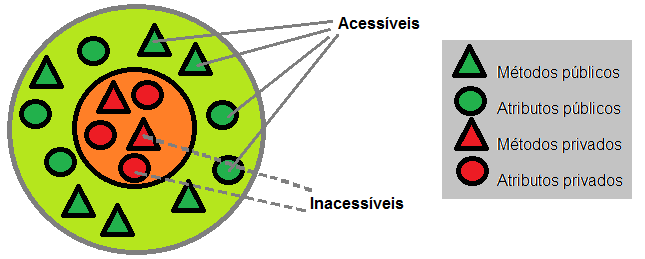
\includegraphics[scale=0.45]{imagens/encapsulamento.png}
  \caption{Encapsulamento}
  \label{fig:encapsulamento}
\end{figure}

\section{Polimorfismo}

É a propriedade que permite que a mesma mensagem seja enviada a diferentes objetos e que cada objeto execute a operação apropriada à sua classe. No caso de polimorfismo, é necessário que os métodos tenham a mesma identificação, utilizado o mecanismo de redefinição de métodos.

No exemplo utilizado na Figura \ref{fig:polimorfismo}, podemos perceber que diferentes objetos, quando é solicitado a mesmo ação, se comportam de maneira diferente. Similar a objetos reais, na Orientação a Objetos, o comportamento por meio do polimorfismo acontece da mesma forma. 

\begin{figure}[H]
  \centering
  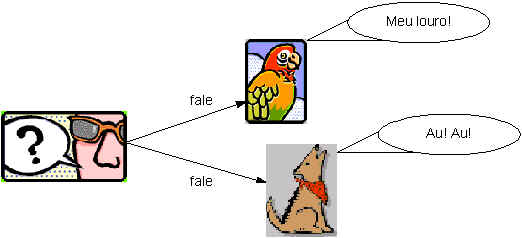
\includegraphics[scale=0.2]{imagens/polianimais.jpg}
  \caption{Polimorfismo}
  \label{fig:polimorfismo}
\end{figure}

\section{Conceitos estudados até este momento}

Para ilustrar, a tabela abaixo contém um resumo e um exemplo de estes conceitos.

\begin{table}[H]
  \resizebox{\textwidth}{!}{%
  \begin{tabular}{|l|l|l|}
  \hline
  \multicolumn{1}{|c|}{\textbf{Palavra-Chave}} & \multicolumn{1}{c|}{\textbf{Breve Definição}} & \multicolumn{1}{c|}{\textbf{Exemplo}} \\ \hline
  Classe & \begin{tabular}[c]{@{}l@{}}Agrupamento de objetos similares que\\ apresentam os mesmos atributos e operações\end{tabular} & Indivíduo, caracterizando as pessoas do mundo \\ \hline
  Atributo & \begin{tabular}[c]{@{}l@{}}Característica particular de uma ocorrência da\\ classe\end{tabular} & \begin{tabular}[c]{@{}l@{}}Indivíduo possui nome, sexo, data de\\ nascimento\end{tabular} \\ \hline
  Operações & \begin{tabular}[c]{@{}l@{}}Lógica contida em uma classe para designar-lhe\\ um comportamento\end{tabular} & \begin{tabular}[c]{@{}l@{}}Cálculo da idade de uma pessoa em uma classe\\ (Indivíduo)\end{tabular} \\ \hline
  Encapsulamento & \begin{tabular}[c]{@{}l@{}}Combinação de atributos e operações de uma\\ classe\end{tabular} & \begin{tabular}[c]{@{}l@{}}Atributo: data de nascimento\\ Operação: cálculo da idade\end{tabular} \\ \hline
  Herança & \begin{tabular}[c]{@{}l@{}}Compartilhamento pela subclasse dos atributos\\ e operações da classe pai\end{tabular} & \begin{tabular}[c]{@{}l@{}}Subclasse (Eucalipto) compartilha atributos e\\ operações da classe (Árvore)\end{tabular} \\ \hline
  Subclasse & Característica particular de uma classe & \begin{tabular}[c]{@{}l@{}}Classe (Árvore),Subclasses (Ipê, Eucalipto,\\ Jacarandá, etc.)\end{tabular} \\ \hline
  Instância de Classe & \begin{tabular}[c]{@{}l@{}}Uma ocorrência específica de uma classe. É o\\ mesmo que objeto\end{tabular} & \begin{tabular}[c]{@{}l@{}}Uma pessoa, uma organização ou um\\ equipamento\end{tabular} \\ \hline
  Objeto & \begin{tabular}[c]{@{}l@{}}Elemento do mundo real (natureza). Sinônimo\\ de instância de classe\end{tabular} & \begin{tabular}[c]{@{}l@{}}Pessoa “Fulano de Tal”, Organização “ACM”,\\ Equipamento “Extintor”\end{tabular} \\ \hline
  Mensagem & \begin{tabular}[c]{@{}l@{}}Uma solicitação entre objetos para invocar certa\\ operação\end{tabular} & Informar idade da pessoa “Fulano de Tal” \\ \hline
  Polimorfismo & \begin{tabular}[c]{@{}l@{}}Habilidade para usar a mesma mensagem para\\ invocar comportamentos diferentes do objeto\end{tabular} & \begin{tabular}[c]{@{}l@{}}Chamada da operação: “Calcular Saldo” de\\ correntista. Invoca as derivações\\ correspondentes para cálculo de saldo de\\ poupança, renda fixa, etc.\end{tabular} \\ \hline
  \end{tabular}%
  }
  \end{table}

  \section*{Exercícios de fixação}

  Baseando-se nas explicações em aula e em suas anotações, responda as seguintes questões:

  \begin{enumerate}
  	\item   Um ponto importante que deve ser claro para podermos atingir o objetivo de nossa disciplina é o conceito sobre classes e objetos. Explique o que são e de exemplos do seu cotidiano para reforçar a ideia.
  	\item O que são atributos e métodos? Defina cada um e de exemplos para afirmar sua resposta.
  	\item Um dos pilares da orientação a objeto é a Herança. Desenho um gráfico, semelhante ao da Figura \ref{fig:heranca}, representado a sua Árvore Genealógica. Caso consiga, vá té seus bisavós. 
  	\item Utilizando a atividade anterior. Identifique os possíveis objetos que podem ser herdados de outros objetos. Utilize setas que apontam do objeto \textbf{Especializado} para o \textbf{Generalizado}. 
  	\item Utilizando a atividade anterior. Represente, por setas, as possíveis trocas de mensagem entre os objetos que você pode identificar. 
  \end{enumerate}
  



  

  



